\documentclass[tikz,border=0mm]{standalone}
\definecolor{iconblue}{RGB}{70,140,255}
\begin{document}
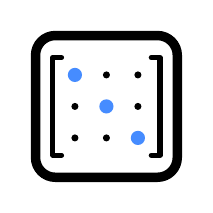
\begin{tikzpicture}[line width=1.2mm,line cap=round,line join=round]
  \useasboundingbox (-1,-1) rectangle (1,1);
  \draw[rounded corners=0.25cm] (-0.9,-0.9) rectangle (0.9,0.9);
  \draw[line width=0.65mm] (-0.57,0.62) -- (-0.68,0.62)
    -- (-0.68,-0.62) -- (-0.57,-0.62);
  \draw[line width=0.65mm] (0.57,0.62) -- (0.68,0.62)
    -- (0.68,-0.62) -- (0.57,-0.62);
  \foreach \i in {0,1,2} {
    \foreach \j in {0,1,2} {
      \ifnum\i=\j
        \fill[iconblue] ({-0.4+0.4*\j},{0.4-0.4*\i}) circle (0.09);
      \else
        \fill[black] ({-0.4+0.4*\j},{0.4-0.4*\i}) circle (0.045);
      \fi
    }
  }
\end{tikzpicture}
\end{document}
